\documentclass[a4paper,10pt]{article}
\usepackage[brazilian]{babel}
\usepackage[left=2.5cm,right=2.5cm,top=3cm,bottom=2.5cm]{geometry}
\usepackage{mathtools}
\usepackage{amsthm}
\usepackage{amsmath}
%\usepackage{nccmath}
\usepackage{amssymb}
\usepackage{amsfonts}
\usepackage{physics}
%\usepackage{dsfont}
%\usepackage{mathrsfs}

\usepackage{titling}
\usepackage{indentfirst}

\usepackage{bm}
\usepackage[dvipsnames]{xcolor}
\usepackage{cancel}

\usepackage{xurl}
\usepackage[colorlinks=true]{hyperref}

\usepackage{float}
\usepackage{graphicx}
%\usepackage{tikz}
\usepackage{caption}
\usepackage{subcaption}

%%%%%%%%%%%%%%%%%%%%%%%%%%%%%%%%%%%%%%%%%%%%%%%%%%%

\newcommand{\eps}{\epsilon}
\newcommand{\vphi}{\varphi}
\newcommand{\cte}{\text{cte}}

\newcommand{\N}{\mathbb{N}}
\newcommand{\Z}{\mathbb{Z}}
\newcommand{\Q}{\mathbb{Q}}
\newcommand{\R}{\vb{R}}
\newcommand{\C}{\mathbb{C}}
\renewcommand{\S}{\hat{S}}
%\renewcommand{\H}{\s{H}}

\renewcommand{\a}{\vb{a}}
\newcommand{\nn}{\hat{n}}
\renewcommand{\d}{\dagger}
\newcommand{\up}{\uparrow}
\newcommand{\down}{\downarrow}

\newcommand{\0}{\vb{0}}
%\newcommand{\1}{\mathds{1}}
\newcommand{\E}{\vb{E}}
\newcommand{\B}{\vb{B}}
\renewcommand{\v}{\vb{v}}
\renewcommand{\r}{\vb{r}}
\renewcommand{\k}{\vb{k}}
\newcommand{\p}{\vb{p}}
\newcommand{\q}{\vb{q}}
\newcommand{\F}{\vb{F}}

\newcommand{\s}{\sigma}
%\newcommand{\prodint}[2]{\left\langle #1 , #2 \right\rangle}
\newcommand{\cc}[1]{\overline{#1}}
\newcommand{\Eval}[3]{\eval{\left( #1 \right)}_{#2}^{#3}}

\newcommand{\unit}[1]{\; \mathrm{#1}}

\newcommand{\n}{\medskip}
\newcommand{\e}{\quad \mathrm{e} \quad}
\newcommand{\ou}{\quad \mathrm{ou} \quad}
\newcommand{\virg}{\, , \;}
\newcommand{\ptodo}{\forall \,}
\renewcommand{\implies}{\; \Rightarrow \;}
%\newcommand{\eqname}[1]{\tag*{#1}} % Tag equation with name

\setlength{\droptitle}{-7em}

\theoremstyle{plain}
\newtheorem{theorem}{Teorema}[section]
%\newtheorem{defi}[theorem]{Definição}
\newtheorem{lemma}[theorem]{Lema}
%\newtheorem{corol}[theorem]{Corolário}
%\newtheorem{prop}[theorem]{Proposição}
%\newtheorem{example}{Exemplo}
%
%\newtheorem{inneraxiom}{Axioma}
%\newenvironment{axioma}[1]
%  {\renewcommand\theinneraxiom{#1}\inneraxiom}
%  {\endinneraxiom}
%
%\newtheorem{innerpostulado}{Postulado}
%\newenvironment{postulado}[1]
%  {\renewcommand\theinnerpostulado{#1}\innerpostulado}
%  {\endinnerpostulado}
%
%\newtheorem{innerexercise}{Exercício}
%\newenvironment{exercise}[1]
%  {\renewcommand\theinnerexercise{#1}\innerexercise}
%  {\endinnerexercise}
%
%\newtheorem{innerthm}{Teorema}
%\newenvironment{teorema}[1]
%  {\renewcommand\theinnerthm{#1}\innerthm}
%  {\endinnerthm}
%
\newtheorem{innerlema}{Lema}
\newenvironment{lema}[1]
  {\renewcommand\theinnerlema{#1}\innerlema}
  {\endinnerlema}
%
%\theoremstyle{remark}
%\newtheorem*{hint}{Dica}
%\newtheorem*{notation}{Notação}
%\newtheorem*{obs}{Observação}


\title{\Huge{\textbf{Lista 3 - Matéria Condensada 2}}}
\author{Mateus Marques}

\begin{document}

\maketitle

\section{Simetrias proibidas e quase-cristais}

(b) Definimos
$$
\boxed{ S(k) = \sum_{n} e^{-i k x_n} } = \sum_{n} e^{-i k (n a)} e^{-i k F(na)}.
$$

Como $f_k(x) = e^{-i k F(x)}$ é uma função periódica de período $b$, podemos escrevê-la como uma série de Fourier, sendo $A_q(k)$ seus coeficientes:
$$
f_k(x) = e^{-i k F(x)} = \sum_{q} A_q(k) \, e^{i \frac{2\pi q x}{b}}, \quad
\boxed{ A_q(k) = \frac{1}{b} \int_0^b e^{-\frac{2\pi i q y}{b}} e^{-i k F(y)} \dd{y}. }
$$

Assim
$$
S(k) = \sum_{n} e^{-i k (n a)} e^{-i k F(na)} = \sum_{q} A_q(k) \sum_{n} e^{-i\qty(k - \frac{2\pi q}{b})(na)}.
$$

Mas lembre que, num Bravais Lattice de $N$ sítios e sendo $\k$ arbitrário, temos (Apêndice F do Ashcroft)
$$
\sum_{\vb{R}} e^{i \k \vdot \vb{R}} = N \sum_{\vb{G}} \delta_{\k,\vb{G}},
$$
onde a soma da esquerda $\sum_{\vb{R}}$ percorre o Bravais Lattice (de $N$ sítios) e a soma da direita $\sum_{\vb{G}}$ percorre o Reciprocal Lattice. Aplicando isso para o nosso caso, temos $\vb{R} = na \vu{x}$, $\vb{G} = \frac{2\pi p}{a} \vu{x}$, com $n, p$ inteiros, de maneira que
$$
\sum_{n} e^{-i \qty(k - \frac{2 \pi q}{b}) (na)} = N \sum_{p} \delta_{\qty(k - \frac{2 \pi q}{b}), \frac{2\pi p}{a}} =
N \sum_{p} \delta_{k, G_{pq}}, \quad G_{pq} = \frac{2\pi p}{a} + \frac{2\pi q}{b}.
$$

Portanto temos que
$$
\boxed{ S(k) = N \sum_{p, q} A_q(k) \, \delta_{k, G_{pq}}. }
$$

(c) Reescrevemos a sequência $x_n$ como
$$
x_n = n + \rho [n \s] = n + \rho ( n \s - \{n\s\}) = n (1 + \rho \s) - \rho \qty{\frac{n (1 + \rho \s)}{(1+\rho\s)/\s}},
$$
onde identificamos $a = (1 + \rho \s)$, $F(x) = -\rho \qty{\frac{x}{b}}$, com $b = \frac{1+\rho\s}{\s}$. Podemos calcular diretamente os coeficientes, fazendo a mudança de variável $z = \frac{y}{b}$:
$$
A_q(k) = \frac{1}{b} \int_0^b e^{-\frac{2\pi i q y}{b}} e^{-i k F(y)} \dd{y} =
\frac{1}{b} \int_0^b e^{-\frac{2\pi i q y}{b}} e^{i k \rho \qty{\frac{x}{b}}} \dd{y} =
\int_0^1 e^{-2\pi i q z} e^{i k \rho \qty{z}} \dd{z},
$$
mas $\qty{z} = z$ para $0 \leq z < 1$, então
$$
A_q(k) = \int_0^1 e^{-i(2\pi q - k \rho) z} \dd{z} =
\frac{1}{-i(2\pi q - k\rho)} \eval{\qty[e^{-i(2\pi q - k \rho) z}]}_{z=0}^{z=1}.
$$

Definindo então $X_{q}(k) = 2\pi q - k \rho$ (só depende de $q$ e $k$), obtemos
$$
A_q(k) = \frac{1}{-i X_q(k)} \qty(e^{-i X_q(k)} - 1) =
\frac{e^{-i X_q(k)/2}}{X_q(k)/2} \cdot \frac{\qty(e^{iX_q(k)/2} - e^{-iX_q(k)/2})}{2i} =
e^{-iX_q(k) / 2} \frac{\sin(X_q(k)/2)}{X_q(k)/2}.
$$

Se agora definirmos $X_{pq} = X_q(k = G_{pq})$, vemos facilmente que $\boxed{ X_{pq} = \frac{2\pi \rho}{(1+\rho\s)}\qty(\frac{q}{\rho} - p) }$ e obtemos
$$
\boxed{ S(k) = \sum_{n} e^{-ikx_n} = N \sum_{p,q} e^{-i X_{pq}/2} \, \frac{\sin(X_{pq}/2)}{X_{pq}/2} \delta_{k, G_{pq}}. }
$$



\pagebreak

\section{Densidade de estados}

(a) A densidade de estados por unidade de volume $d-$dimensional $V$ é
$$
\rho(E) = \frac{1}{V} \sum_{\k, \s} \delta(E - \eps(\k)) = \frac{2}{V} \cdot \frac{V}{(2\pi)^d} \int_{\R^d} \dd[d]{\k} \delta(E - \eps(\k)) = \frac{2}{(2\pi)^d} \int_{\R^d} \dd[d]{\k} \delta(E - \eps(\k)).
$$

Como pode ser visto na página \href{https://en.wikipedia.org/wiki/Dirac_delta_function#Properties}{$\delta$ de Dirac da Wikipédia}, vale a seguinte identidade
$$
\int_{\R^n} f(\r) \delta(g(\r)) \dd[n]{\r} = \int_{g^{-1}(0)} \frac{f(\r)}{\abs{\grad{g(\r)}}} \dd{\s(\r)},
$$
onde a expressão da direita é uma integral sobre a superfície $(n-1)-$dimensional $g^{-1}(0)$ (pontos $\r$ tais que $g(\r) = 0$). Dessa maneira
$$
\rho(E) = \frac{2}{(2\pi)^d} \int_{\eps^{-1}(E)} \frac{\dd{\s(\k)}}{\abs{\eps(\k)}} =
\frac{2}{(2\pi)^d} \int_{C(E)} \frac{\dd{\s(\k)}}{\abs{\grad{\eps(\k)}}},
$$
onde $C(E) = \eps^{-1}(E)$ é a superfície de Fermi. No caso $d = 2$ temos uma integral de linha:
$$
\rho(E) = \frac{1}{2\pi^2} \int_{C(E)} \frac{\dd{\ell}}{\abs{\grad{\eps(\k)}}}.
$$

Expandindo $\eps(\k)$ em segunda ordem em Taylor ao redor de um ponto crítico $\k_o = (k_{xo}, k_{yo})$, podemos rotacionar $(k_x, k_y)$ de maneira que o termo de derivada mista $\pdv{\eps}{k_x}{k_y}$ seja zero. Dessa maneira, sem perda de generalidade temos
$$
\eps(\k) \approx \eps_o + \frac{A}{2} \qty[(k_x - k_{xo})^2 + \zeta (k_y - k_{yo})^2],
$$
onde $(A, \zeta) = (+1, +1)$ corresponde a um ponto de mínimo, $(A, \zeta) = (-1, +1)$ ponto de máximo e $(A, \zeta) = (+1, -1)$ a um ponto de sela (equivalente a $(A, \zeta) = (-1, +1)$).

Nos casos de ponto de máximo e mínimo, a superfície $C(\eps)$ é um círculo de raio $R = \sqrt{2\abs{\eps-\eps_o}}$, pois
$$
(k_x - k_{xo})^2 + (k_y - k_{yo})^2 = 2 \abs{\eps - \eps_o} = R^2,
$$
com $\eps < \eps_o$ para ponto de máximo e $\eps > \eps_o$ para ponto de mínimo. Portanto, nesses dois casos $\abs{\grad{\eps(\k)}} = \sqrt{(k_x - k_{xo})^2 + (k_y - k_{yo})^2} = R$, $\dd{\ell} = R \dd{\theta}$ e
$$
\rho(E) = \frac{1}{2\pi^2} \int_0^{2\pi} \frac{R \dd{\theta}}{R} = \frac{1}{\pi} = \cte.
$$

Para calcular o caso do ponto de sela $(A, \zeta) = (+1, -1)$, acho mais fácil utilizar a expressão do $\delta$ de Dirac para a densidade de estados:
$$
\rho(E) = \frac{1}{2\pi^2} \int_{\R^2} \dd[2]{\k} \delta(E - \eps(\k)) =
\frac{4}{2 \pi^2} \int_0^K \dd{q_y} \int_0^\infty \dd{q_x}
\delta\qty(\abs{E - \eps_o} + \frac{q_y^2}{2} - \frac{q_x^2}{2}),
$$
onde a integração é sobre a variável $\q = \k - \k_o$, o fator $4$ apareceu devido à simetria entre os quadrantes $(\pm q_x, \pm q_y)$ e foi introduzido um cutoff $K$ para que a integral não divirja e possamos analisar seu comportamento.

Usando que $\displaystyle{\delta(g(x)) = \sum_{g(a)=0} \frac{1}{\abs{g'(a)}} \delta(x-a)}$ e $\displaystyle{\int \frac{\dd{x}}{\sqrt{x^2+a}} = \log(x + \sqrt{x^2 + a})}$ (Mathematica), temos
$$
\rho(E) = \frac{2}{\pi^2} \int_0^K \frac{\dd{q_y}}{\sqrt{q_y^2 + 2 \abs{E-\eps_o}}} =
\text{constante} - \frac{1}{\pi^2} \log\abs{E-\eps_o}.
$$

\textbf{FALTA ESBOÇAR OS TRÊS (DOIS) CASOS, CONSTANTE E DIV LOGARITMICA.}

\textbf{TALVEZ CORRIGIR A CONSTANTE QUE ACOMPANHA O LOG.}

\n

(b) Temos que $E(\k) = \sqrt{\xi^2(\k) + \Delta^2}$. Assim, uma quase-partícula com energia $E$ corresponde a dois estados, um com energia $\xi_+ = \sqrt{E^2 - \Delta^2}$ e outro com $\xi_- = -\sqrt{E^2 - \Delta^2}$. Assim, temos que
$$
g(E) \dd{E} = \rho(\xi_+) \abs{\dd{\xi_+}} + \rho(\xi_-) \abs{\dd{\xi_-}}.
$$

Supondo que $E > \Delta$ e $-D < \xi_\pm < D$, temos então que
$$
g(E) = \rho(\xi_+) \abs{\dv{\xi_+}{E}} + \rho(\xi_-) \abs{\dv{\xi_-}{E}} =
\frac{1}{D} \, \qty(\abs{\frac{2E}{2\sqrt{E^2-\Delta^2}}} + \abs{\frac{-2E}{2\sqrt{E^2-\Delta^2}}}) \implies
$$
$$
\boxed{ g(E) = \frac{2 \abs{E}}{D \sqrt{E^2 - \Delta^2}}. }
$$

\textbf{FALTA ESBOÇAR O GRÁFICO DE $g(E)$ E DISCUTIR O RESULTADO.}

\textbf{RELACIONAR O GAP SUPERCONDUTOR COM A TEORIA DE BANDAS.}


\url{https://physics.stackexchange.com/questions/266965/what-is-the-difference-of-the-gap-between-superconductor-and-insulator}

In a conventional conductor any momentum eigenstate in the band can be occupied by at most two electrons (with opposite spins) so in a full band the net momentum of the electrons in the band is zero i.e. there is no net drift velocity and hence no current.

In a superconductor the electrons pair up into Cooper pairs that obey Bose-Einstein statistics, so any number of Cooper pairs can occupy the same momentum state. That means the electrons joined into Cooper pairs can have a net momentum, and hence a net drift velocity, so they can carry a current.

Existence of a gap means that ground state and excited states are well separated and a transition from ground state and excited states requires some energy.

Existence of a gap does not determine whether a system is insulating or not. In your case, conductivity is determined by the ground state. For an insulator, the ground state is insulating while ground state of superconductor is superconducting. A gap here means it is not easy for insulator to be excited to carry currents and for superconductors to lose its superconductivity.



\pagebreak

\section{Elétrons de Bloch}

A hamiltoniana de Bloch é
$$
H_{\k} = -\frac{\hbar^2}{2m} \qty[\laplacian + 2i \k \vdot \grad - \k \vdot \k].
$$
Calculando $H_{\k + \q}$, obtemos
$$
H_{\k + \q} = -\frac{\hbar^2}{2m} \qty[\laplacian + 2i (\k + \q) \vdot \grad - (\k + \q) \vdot (\k + \q)] =
H_{\k} - \frac{\hbar^2}{2m} \qty[2 i \q \vdot \grad - 2 \q \vdot \k - q^2]
$$
$$
H_{\k + \q} = H_{\k} + V, \quad \boxed{V = \frac{\hbar^2}{m} \q \vdot \qty(-i \grad + \k) + \frac{\hbar^2}{2m} \, q^2.}
$$

Seguindo o Apêndice E do Ashcroft, iremos calcular $\pdv{\eps_n}{k_i}$ e $\pdv{\eps_n}{k_i}{k_j}$ através de teoria de perturbação:
$$
\eps_n(\k+\q) = \eps_n(\k) + \sum_{i} \pdv{\eps_n}{k_i} q_i +
\frac{1}{2} \sum_{i,j} \pdv{\eps_n}{k_i}{k_j} q_i q_j + O(q^3) =
$$
$$
= \eps_n(\k) + \ev{V}{u_{n\k}} + \sum_{n' \neq n} \frac{\abs{\mel{u_{n\k}}{V}{u_{n'\k}}}^2}{\eps_n(\k) - \eps_{n'}(\k)} + \cdots,
$$
onde $\ket{u_{n\k}}$ (com $\braket{\r}{n\k} = \psi_{n\k}(\r) = e^{i\k\vdot\r} u_{n\k}(\r)$) são os autoestados da hamiltoniana de Bloch $H_{\k}$.

\n

(a) O único termo linear de $V$ é $\frac{\hbar^2}{m} \q \vdot (-i\grad + \k)$, portanto
$$
\sum_{i} \pdv{\eps_n}{k_i} q_i = \frac{\hbar^2}{m} \ev{ \q \vdot (-i\grad + \k)}{u_{n\k}} =
\frac{\hbar^2}{m} \int \dd[d]{\r} u_{n\k}^*(\r) \qty[\sum_{i}\qty(-i\grad + \k)_i q_i] u_{n\k}(\r) =
$$
$$
\sum_{i} \pdv{\eps_n}{k_i} q_i =\sum_{i} \qty[\frac{\hbar^2}{m} \int \dd[d]{\r} u_{n\k}^*(\r) \qty(-i\grad + \k)_i u_{n\k}(\r) ] q_i.
$$

Mas note que $\psi_{n\k}^*(\r) \qty(-i\grad) \psi_{n\k}(\r) = u_{n\k}^*(\r) \qty(-i\grad + \k) u_{n\k}(\r)$, portanto
$$
\boxed{\frac{1}{\hbar} \pdv{\eps_n}{\k} = \frac{1}{m} \int \dd[d]{\r} \psi_{n\k}^*(\r) \qty(-i \hbar \grad) \psi_{n\k}(\r) =
\frac{1}{m} \ev{\hat{p}}{n\k} = \v_n(\k),}
$$
que é a velocidade média de um elétron de Bloch no estado $\ket{n\k}$.

\n

(b) $\frac{\hbar^2}{2m} q^2$ (aplicando perturbação de primeira ordem) e $\frac{\hbar^2}{m} \q \vdot (-i\grad + \k)$ (aplicando perturbação de segunda ordem) dão origem a dois termos $O(q^2)$:
$$
\frac{1}{2} \sum_{i,j} \pdv{\eps_n}{k_i}{k_j} q_i q_j =
\sum_{i,j} \frac{\hbar^2}{2m} \, \delta_{ij} q_i q_j +
\sum_{n' \neq n} \frac{\abs{\mel{n\k}{\frac{\hbar^2}{m} \q \vdot (-i\grad)}{n'\k}}^2}{\eps_n(\k) - \eps_{n'}(\k)}.
$$

Podemos ainda reescrever
$$
\abs{\mel**{n\k}{\frac{\hbar^2}{m} \q \vdot (-i\grad)}{n'\k}}^2 =
\sum_{i,j} \qty[ \sum_{n'\neq n}
\mel**{n\k}{\frac{\hbar^2}{m} (-i\grad)_i}{n'\k} \mel**{n'\k}{\frac{\hbar^2}{m} (-i\grad)_j}{n\k} ] q_i q_j =
$$
$$
\frac{\hbar^4}{2 m^2} \sum_{\substack{i,j \\ n' \neq n}}
\qty[
\mel**{n\k}{-i\pdv{r_i}}{n'\k} \mel**{n'\k}{-i\pdv{r_j}}{n\k} +
\mel**{n\k}{-i\pdv{r_j}}{n'\k} \mel**{n'\k}{-i\pdv{r_i}}{n\k}
] q_i q_j.
$$

Finalmente, obtemos
$$
\boxed{\frac{1}{\hbar^2} \pdv{\eps_n}{k_\mu}{k_\nu} = \frac{1}{m} \delta_{\mu\nu} + \qty(\frac{\hbar}{m})^2 \sum_{n'\neq n}
\frac{
\mel**{n\k}{\frac{1}{i}\pdv{r_\mu}}{n'\k} \mel**{n'\k}{\frac{1}{i}\pdv{r_\nu}}{n\k} +
\mel**{n\k}{\frac{1}{i}\pdv{r_\nu}}{n'\k} \mel**{n'\k}{\frac{1}{i}\pdv{r_\mu}}{n\k}
}{\eps_n(\k) - \eps_{n'}(\k)}.}
$$


\pagebreak

\section{Modelos tight-binding}

Farei o cálculo de tight-binding para a rede cúbica em $d$ dimensões. Sendo $\a_j$ ($j=1,2,\ldots,d$) os vetores do Bravais lattice, temos que a hamiltoniana pode ser escrita como
$$
H = -t \sum_{\vb{R}} \sum_{j=1}^{d}
\qty[ c_{(\R+\a_j)}^\d c_{\R} + c_{\R}^\d c_{(\R+\a_j)} ].
$$
Tomando as transformadas de Fourier $c_{(\R+\a_j)}^\d = \frac{1}{\sqrt{N}} \sum_{\k} e^{-i\k\vdot(\R+\a_j)} c_{\k}^\d$ e $c_{\R} = \frac{1}{\sqrt{N}} \sum_{\k'} e^{i\k'\vdot\R} c_{\k'}$, temos
$$
H = \frac{-t}{N} \sum_{\k,\k'} \sum_{j=1}^{d}
\qty{
\cancelto{\boxed{= N \delta_{\k, \k'}}}{\qty[\sum_{\R} e^{-i(\k-\k')\vdot\R}]}
e^{-i\k\vdot\a_j} c_{\k}^\d c_{\k'} + h.c.} =
$$
$$
= -t \sum_{\k} \sum_{j=1}^{d} \qty(e^{i\k\vdot\a_j} + e^{-i\k\vdot\a_j})
c_{\k}^\d c_{\k} =
\sum_{\k} \qty[- 2t \sum_{j=1}^{d} \cos(\k \vdot \a_j)] c_{\k}^\d c_{\k}.
$$

(a) Assim, a relação de dispersão para $d$ dimensões é $\eps(\k) = -2t \sum_{j=1}^{d} \cos(\k \vdot \a_j)$. No caso $d=1$ temos $\boxed{\eps(k) = -2t \cos(ka),}$ e no caso $d = 2$ temos $\boxed{\eps(k_x, k_y) = -2t [\cos(k_x a) + \cos(k_y a) ].}$

\n

Em $d = 1$, como o mínimo de $\eps(\k)$ é $-2t$ e o máximo é $+2t$, a largura de banda é $4t$. Para calcular $\rho(E)$, usando $\displaystyle{\sum_{\k} \to \frac{V}{(2\pi)^d} \int_{\text{BZ}} \dd[d]{\k}}$ e $\displaystyle{\delta(g(x)) = \sum_{g(a)=0} \frac{1}{\abs{g'(a)}} \delta(x-a)}$, temos
$$
\rho(E) = \frac{1}{V} \sum_{\k, \s} \delta(E - \eps(\k)) =
\frac{2}{2\pi} \int_{-\frac{\pi}{a}}^{\frac{\pi}{a}} \delta(E + 2t \cos(ka)) \dd{k} =
\frac{1}{\pi a} \int_{-\pi}^{\pi} \delta(E + 2t \cos(z)) \dd{z} \implies
$$
$$
\rho(E) = \frac{1}{\pi a} \cdot \frac{2}{2t \sin(\arccos(\frac{E}{2t}))} =
\frac{1}{\pi a t \sqrt{1 - \qty(\frac{E}{2t})^2}}.
$$

As singularidades de Van Hove ocorrem quando $\pdv{\eps}{k} = 0$, ou seja, quando $\sin(ka) = 0 \implies k = 0, \pm\frac{\pi}{a}$. Em $k = 0$ temos um mínimo (correspondente a $E = -2t$) e para $k = \pm \frac{\pi}{a}$ temos máximos ($E = 2t$). Como vemos na Figura \ref{fig:tightbinding-d1} abaixo, temos divergências para os dois valores $E = \pm 2t$, onde $\rho(E) \propto \frac{1}{\sqrt{(2t)^2 - E^2}}$.

\begin{figure}[H]
\centering
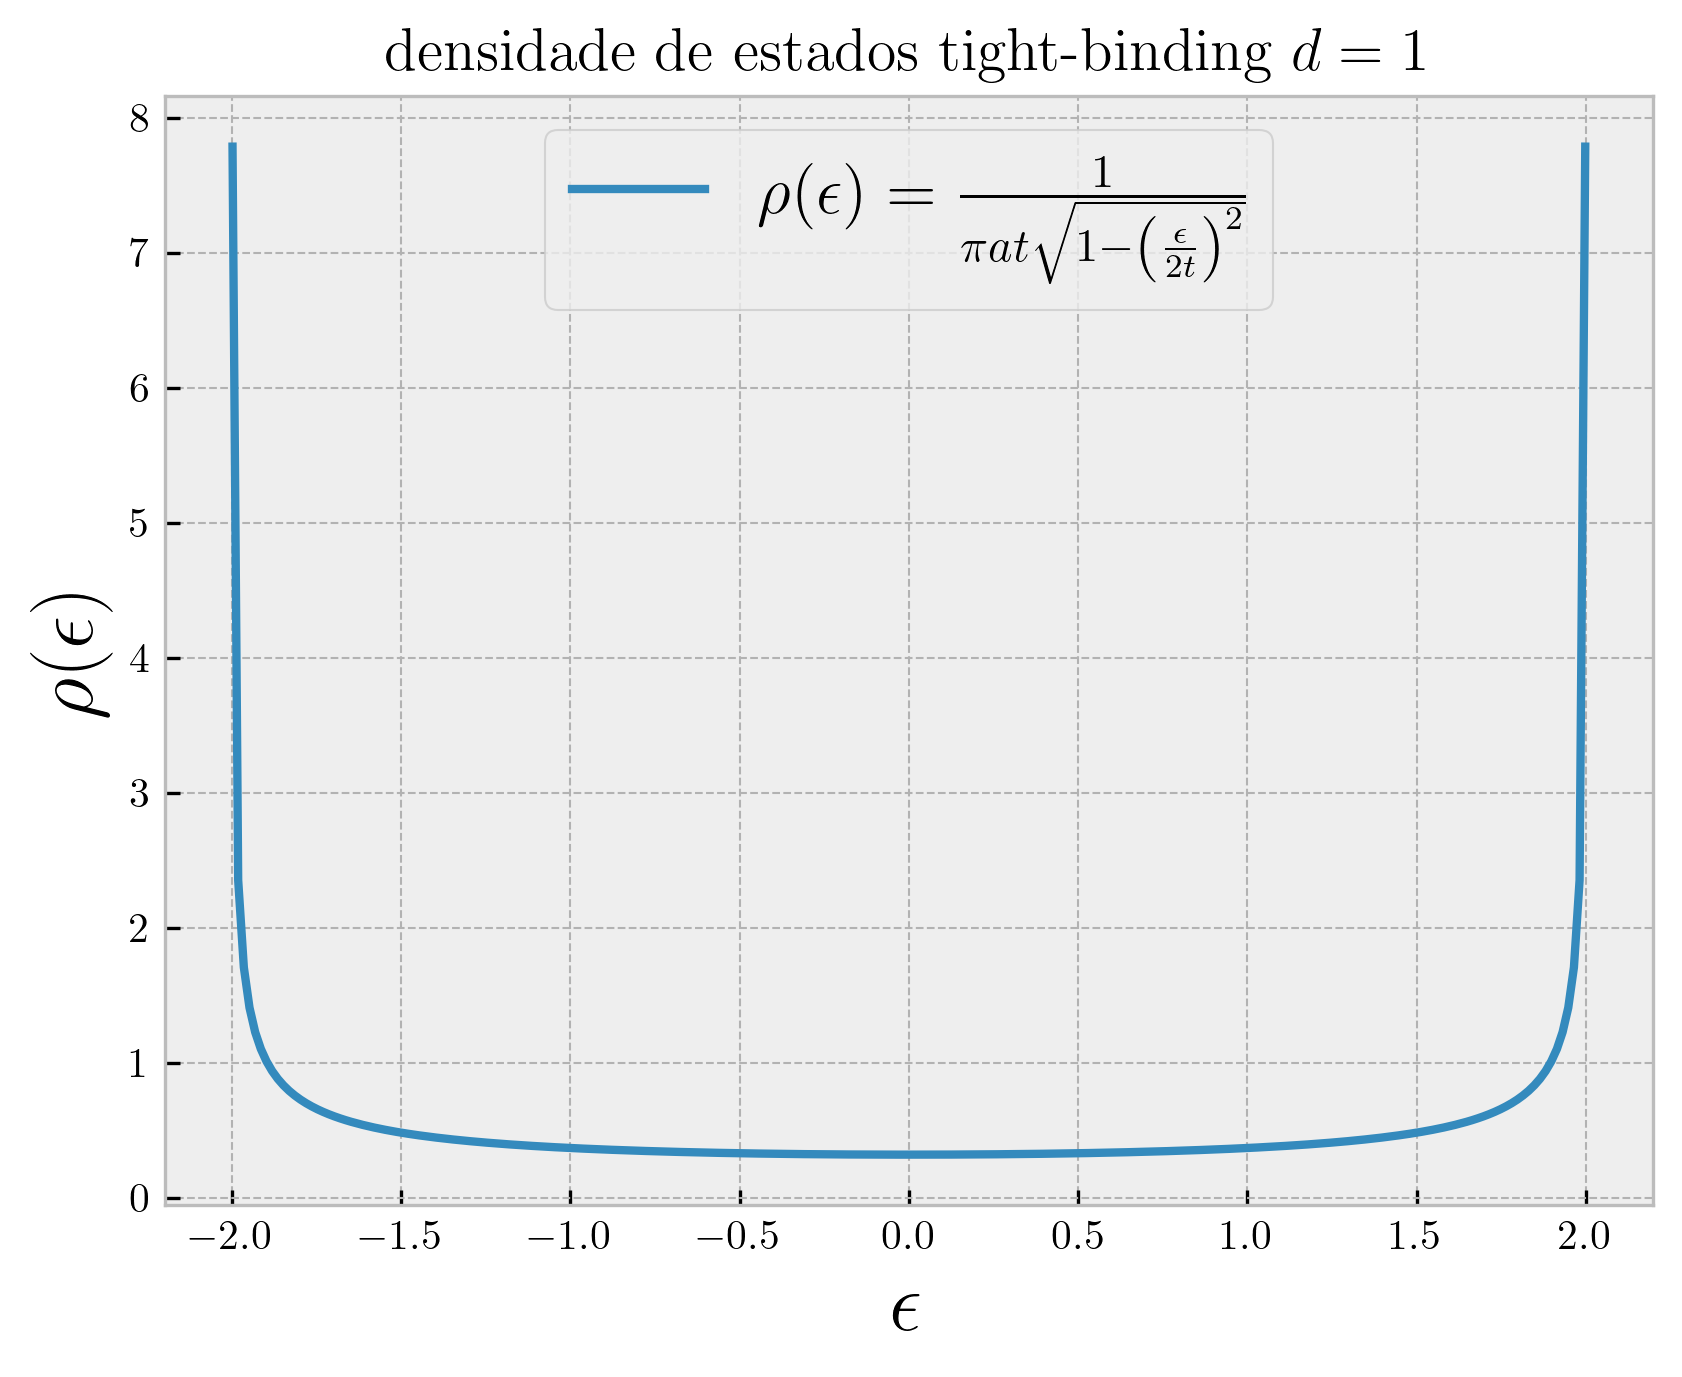
\includegraphics[width=0.6\linewidth]{fig/dos-tightbinding-d1.png}
\caption{Densidade de estados tight-binding para $d=1$. Parâmetros $a = t =1$.}
\label{fig:tightbinding-d1}
\end{figure}

(b) Para $d = 2$ a relação de dispersão é $\eps(k_x, k_y) = -2t [\cos(k_x a) + \cos(k_y a)]$. Seu mínimo é $-4t$ e seu máximo $+4t$, logo a largura de banda é $8t$.


\pagebreak

\section{Instabilidade de Peierls e modelo de Su-Schrieffer-Heeger}

(a) A hamiltoniana do modelo é dada por
$$
H = H_{\text{K}} + H_{\text{el}},
\quad
H_{\text{K}} = -t \sum_{j,\s} (1 + u_j) \qty(c_{j,\s}^\d c_{j+1, \s} + \text{h.c.}),
\quad
H_{\text{el}} = \frac{\kappa}{2} \sum_{j} (u_{j+1} - u_j)^2,
$$
onde $H_{\text{K}}$ é a parte cinética e $H_{\text{el}}$ é a parte elástica.

Considerando a modulação periódica $u_j = (-1)^j \alpha$, temos que $(u_{j+1} - u_j)^2 = 4 \alpha^2$, e portanto a parte elástica é muito simples $H_{\text{el}} = 2 \kappa \alpha^2 N$, onde $N$ é o número (par) de sítios.

Já a parte cinética pode ser diagonalizada considerando duas sub-redes $\textcolor{red}{A}$ (\textcolor{red}{vermelha}, $\textcolor{red}{a_{j,\s}^\d}$ e $\textcolor{red}{a_{j,\s}}$) e $\textcolor{blue}{B}$ (\textcolor{blue}{azul}, $\textcolor{blue}{b_{j,\s}^\d}$ e $\textcolor{blue}{b_{j,\s}}$). Pensando bem, a hamiltoniana cinética então pode ser escrita como
$$
H_{\text{K}} = -w \sum_{j, \s} \qty(a_{j+1,\s}^\d b_{j,\s} + \text{h.c.})
-v \sum_{j,\s} \qty(a_{j,\s}^\d b_{j,\s} + \text{h.c.}),
$$
onde $v = t(1+\alpha)$ é o intra-hopping (entre a mesma célula) e $w = t(1-\alpha)$ é o inter-hopping (entre células diferentes). Supondo que a distância entre duas células unitárias seja $2a$, as transformadas de Fourier são
$$
a_{j,\s}^\d = \frac{1}{\sqrt{N}} \sum_{k} e^{-ik (2a) j} a_{k,\s}, \quad
b_{j,\s}^\d = \frac{1}{\sqrt{N}} \sum_{k'} e^{-ik' (2a) j} b_{k',\s}.
$$

Substituindo em $H_{\text{K}}$, temos
$$
H_{\text{K}} = - \frac{1}{N}
\sum_{j,\s} \qty{ v
\sum_{k,k'} e^{-ik(2a)(j+1)} e^{ik'(2a)j} a_{k,\s}^\d b_{k',\s}
+ w
\sum_{k,k'} e^{-ik(2a)j} e^{ik'(2a)j} a_{k,\s}^\d b_{k',\s}} + \text{h.c.} =
$$
$$
= - \frac{1}{N}
\sum_{k, k', \s} \qty{ v
\cancelto{\boxed{N \delta_{k,k'}}}{\qty[\sum_{j} e^{-i(k-k')(2a)j}]}
e^{-ik(2a)} a_{k,\s}^\d b_{k',\s}
+ w
\cancelto{\boxed{N \delta_{k,k'}}}{\qty[\sum_{j} e^{-i(k-k')(2a)j}]}
a_{k,\s}^\d b_{k',\s}} + \text{h.c.} =
$$
$$
= - \sum_{k, \s} \qty{ \qty[ w  + v
e^{-ik(2a)}]
a_{k,\s}^\d b_{k,\s} + \text{h.c.} } =
- \sum_{k, \s} \qty{ \qty[ w  + v
e^{-ik(2a)}]
a_{k,\s}^\d b_{k,\s} +
\qty[ w  + v
e^{ik(2a)}]
b_{k,\s}^\d a_{k,\s}
} =
$$
$$
= \sum_{k, \s}
\begin{pmatrix}
a_{k,\s}^\d & b_{k,\s}^\d
\end{pmatrix}
\begin{pmatrix}
0 & -w - v e^{-2ika} \\
-w - v e^{+2ika} & 0
\end{pmatrix}
\begin{pmatrix}
a_{k,\s} \\ b_{k,\s}
\end{pmatrix}.
$$

Portanto, as energias da parte cinética são $\eps_\pm(k) = \pm \sqrt{\abs{w + v e^{2ika}}^2} = \pm \sqrt{w^2 + v^2 + 2 vw \cos(2ka)}$. Como a distância entre células unitárias é $2a$, a zona de Brillouin é $-\frac{\pi}{2a} \leq k < \frac{\pi}{2a}$.

Fazendo os gráficos somente da parte cinética (a elástica é uma constante), temos a Figura \ref{fig:eps-ssh}:
\begin{figure}[H]
\centering
\begin{subfigure}{.45\textwidth}
  \centering
  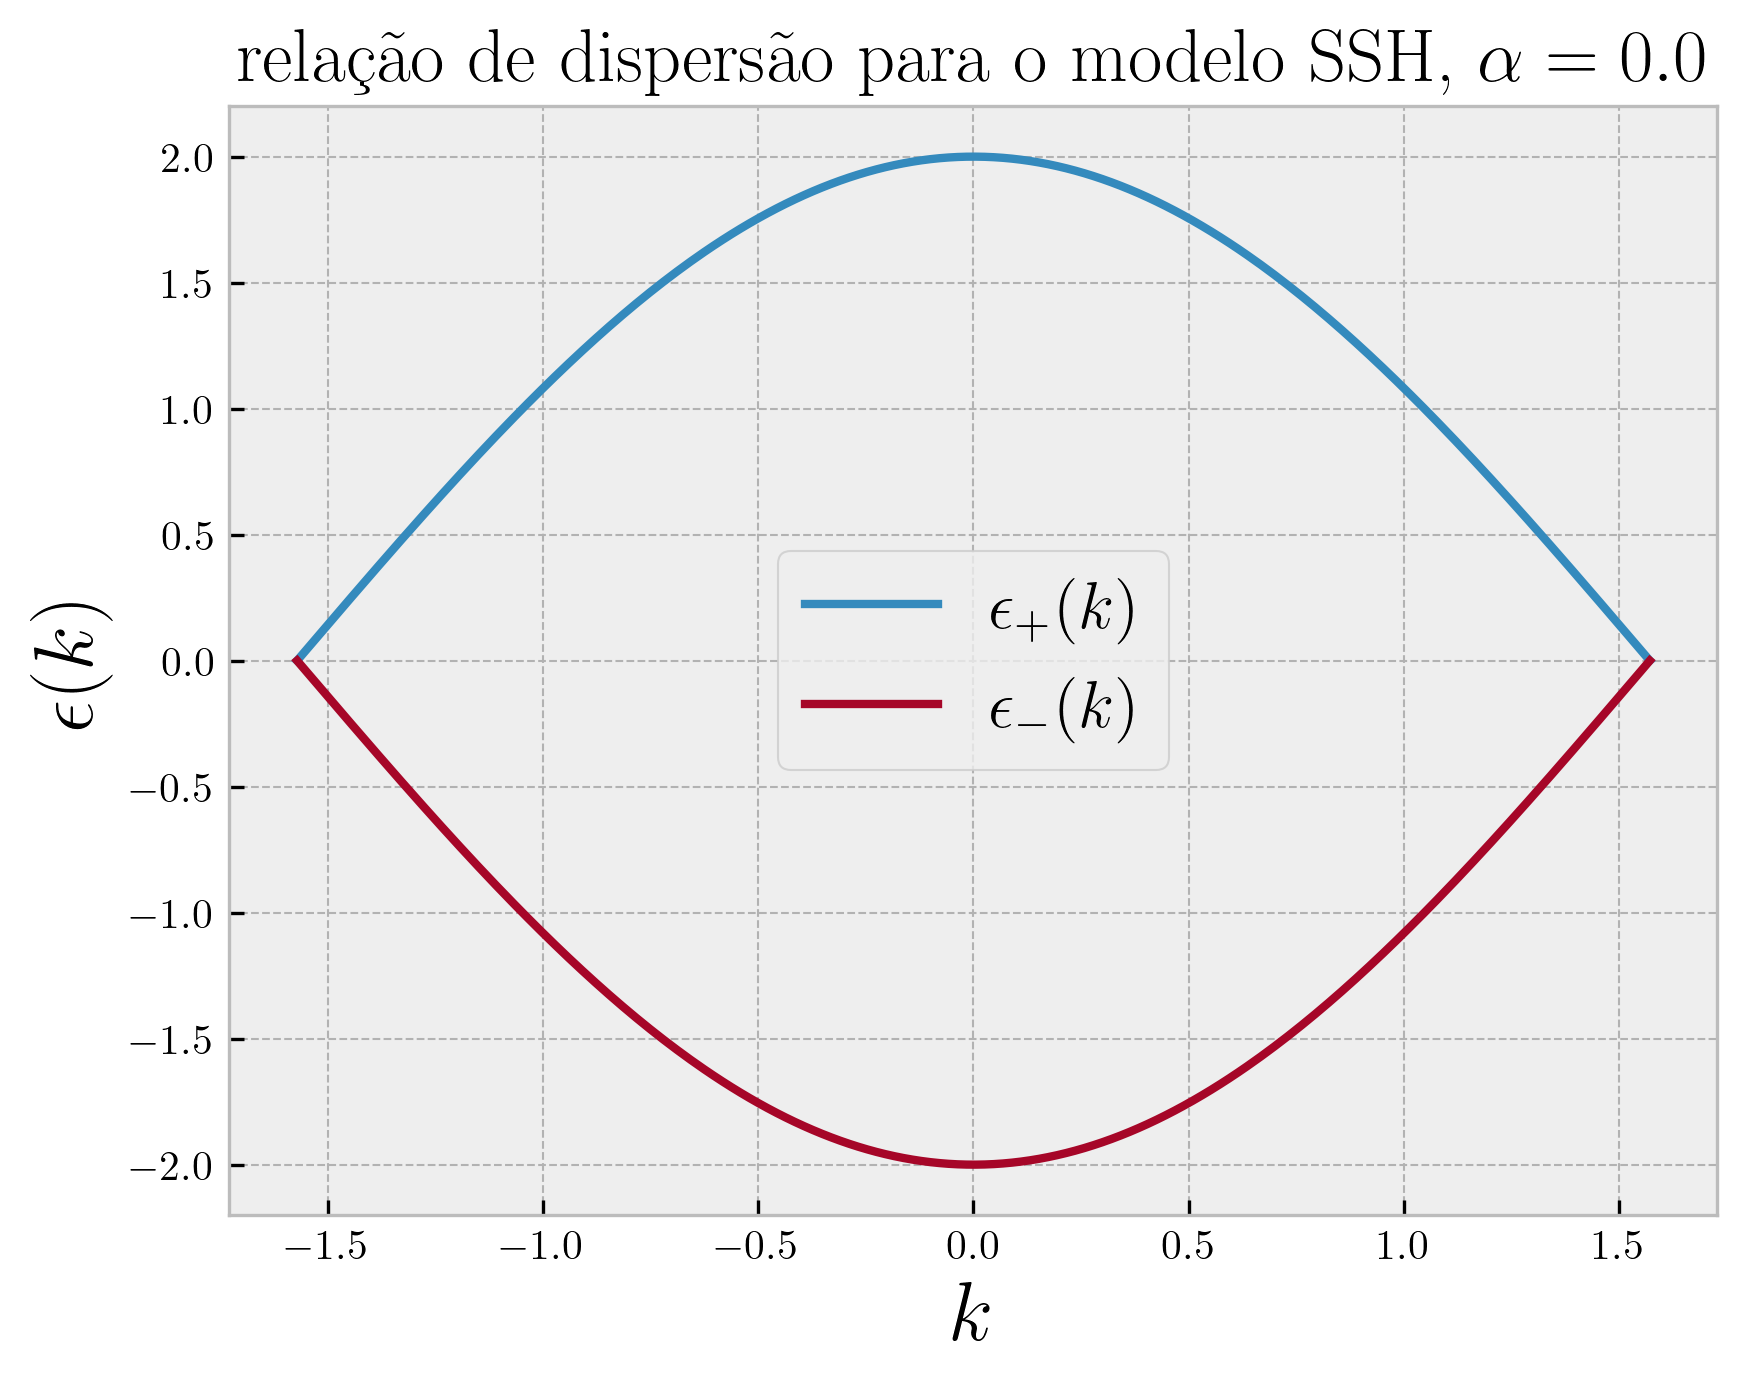
\includegraphics[width=\linewidth]{fig/eps_ssh_alpha0.png}
  \label{fig:ssh-alpha0}
\end{subfigure}
\begin{subfigure}{.45\textwidth}
  \centering
  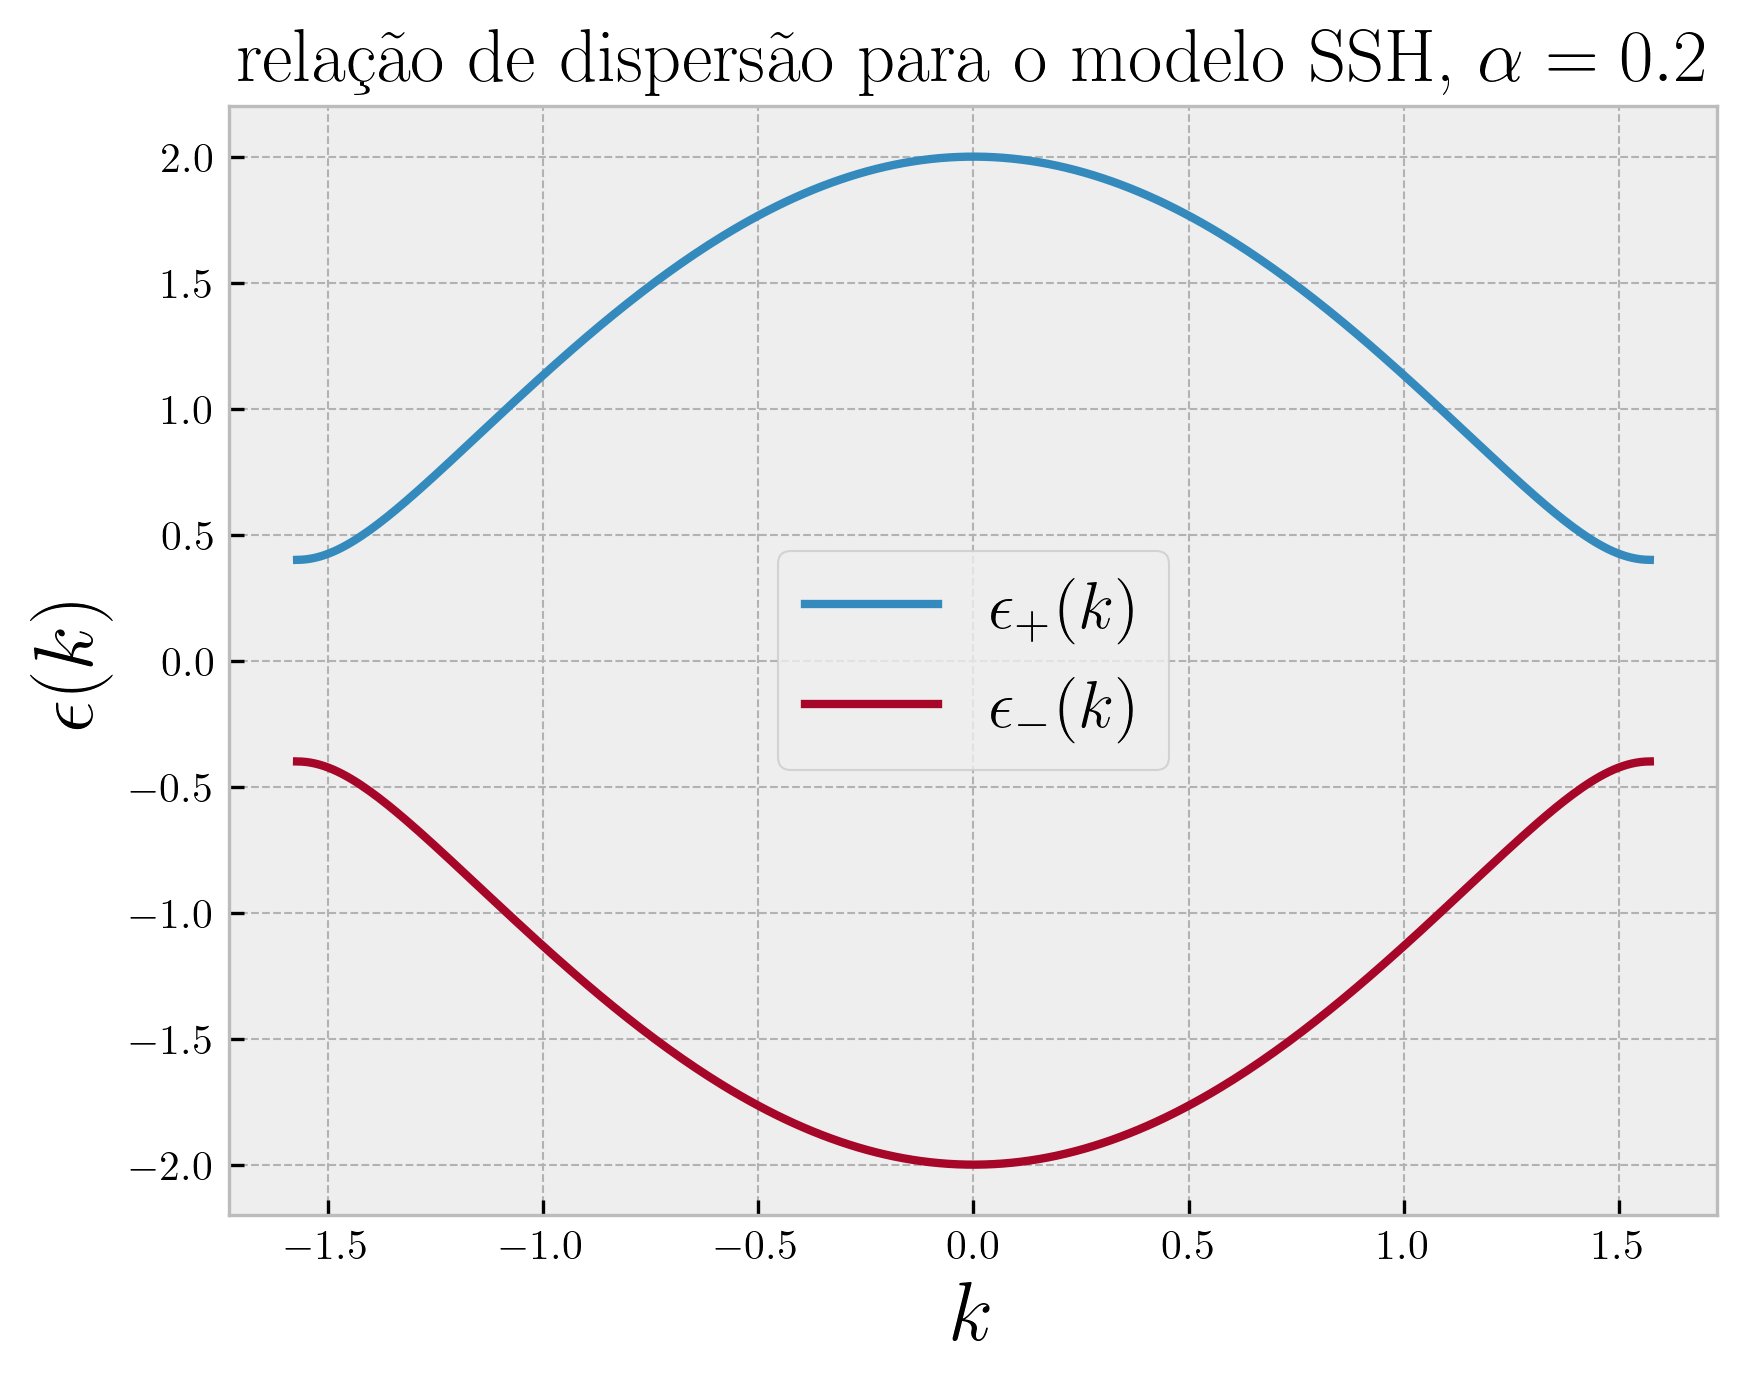
\includegraphics[width=\linewidth]{fig/eps_ssh_alphanot0.png}
  \label{fig:ssh-alphanot0}
\end{subfigure}
\caption{Relação de dispersão do modelo SSH para $\alpha = 0$ e $\alpha = 0.2$. Parâmetros $a = t = 1$.}
\label{fig:eps-ssh}
\end{figure}

(b) Para a energia do sistema em $T = 0$ temos
$$
E = \int_{-\infty}^{E_F} \eps \rho(\eps) \dd{\eps},
$$
onde a densidade de estados (incluindo as duas bandas $n = +$ e $n = -$) é
$$
\rho(\eps) = \sum_{n} \sum_{k, \s} \delta(\eps - \eps_n(k)) =
\frac{2 \cdot \cancelto{\boxed{2a}}{V}}{2\pi}
\sum_{n} \int_{\text{BZ}} \delta(\eps - \eps_n(k)) \dd{k}.
$$

Assim
$$
E = \frac{2a}{\pi} \sum_{n} \int_{\text{BZ}} \dd{k}
\int_{-\infty}^{E_F} \eps \, \delta(\eps - \eps_n(k)) \dd{\eps} =
\frac{2a}{\pi} \sum_{n < E_F} \int_{\text{BZ}} \eps_n(k) \dd{k},
$$
onde só integramos as bandas com energia menor que a energia de Fermi $E_F$. Na situação de semipreenchimento, só consideramos a banda $n=-$ com dispersão $\eps_-(k)$. Usando $\cos(2\xi) = 1 - 2 \sin[2](\xi)$ e a integral elíptica dada no exercício:
$$
E = - \frac{2a}{\pi} \int_{-\frac{\pi}{2a}}^{\frac{\pi}{2a}}
t \sqrt{2 \, \qty[1 + \alpha^2 + (1-\alpha^2) \cos(2ka)]} \dd{k} =
- \frac{4t}{\pi} \int_{-\frac{\pi}{2}}^{\frac{\pi}{2}}
\qty[1 - (1-\alpha^2) \sin[2](\xi)]^{1/2} \dd{\xi} \implies
$$
$$
E \simeq -\frac{4t}{\pi}
\qty[2 + (a_1 - b_1 \ln \alpha^2) \alpha^2]
$$

A energia total é
$$
U =
\qty{2\kappa \alpha^2 -\frac{4t}{\pi}
\qty[2 + (a_1 - b_1 \ln \alpha^2) \alpha^2]} N.
$$

Mostrar que
$$
\eval{\dv{U}{\alpha}}_{\alpha=0} = 0,
$$
$$
\eval{\dv[2]{U}{\alpha}}_{\alpha=0} =
2 \eval{\dv{U}{\alpha^2}}_{\alpha=0}
= 0.
$$

Elliptic approximation \url{https://math.stackexchange.com/questions/1093786/approximation-for-elliptic-integral-of-second-kind}.

\n\n

(c) Fazer desenho dos dois padrões de dimerização. Só desenhar as cadeias, com os edges states no caso não-trivial.

\n\n

(d) Mostrar que esse
$$
\Psi = \frac{1}{\sqrt{2}} \begin{pmatrix}
1 \\ -e^{i\vphi_k}
\end{pmatrix}
$$
é autovetor da matriz lá com $w + ve^{\pm 2ika}$.


\end{document}
